\documentclass[a4paper,10pt]{article}

% Hier die Nummer des Blatts und Autoren angeben.
\newcommand{\blatt}{1}
\newcommand{\autor}{Merlin Steuer}

\usepackage{hci}

\begin{document}
% Seitenkopf mit Informationen
\kopf
\renewcommand{\figurename}{Figure}

\aufgabe{1}

\begin{enumerate}
	\item Es ergeben sich folgende Anforderungen: \begin{itemize}
		\item Das Gerät muss Wasserdicht sein
		\item Das Gerät muss Temperaturen weit unter 0 Grad aushalten		
		\item Gute Sichtbarkeit der nötigen Informationen auf dem Display
		\item Die Menüführung soll komplett mittels mechanischer Eingabeelemente möglich sein
		\item Ein großes (Touch-)Display mit starker Hintergrundbeleuchtung sollte die Zentrale Bedieneinheit darstellen
		\item Zieleingabe in Form von Koordinaten (per Bildschirmtastatur) soll möglich sein
		\item Während der Fahrt soll eine Möglichkeit bestehen, schnell die Karte zu zoomen oder den sichtbaren Kartenausschnitt zu verändern
		\item Das Gerät soll auch mit dickeren Handschuhen Bedienbar bleiben 
		\item Die Akkulaufzeit sollte mindestens 8 Stunden betragen
	\end{itemize}
	\item Siehe folgende Abbildung:
		
	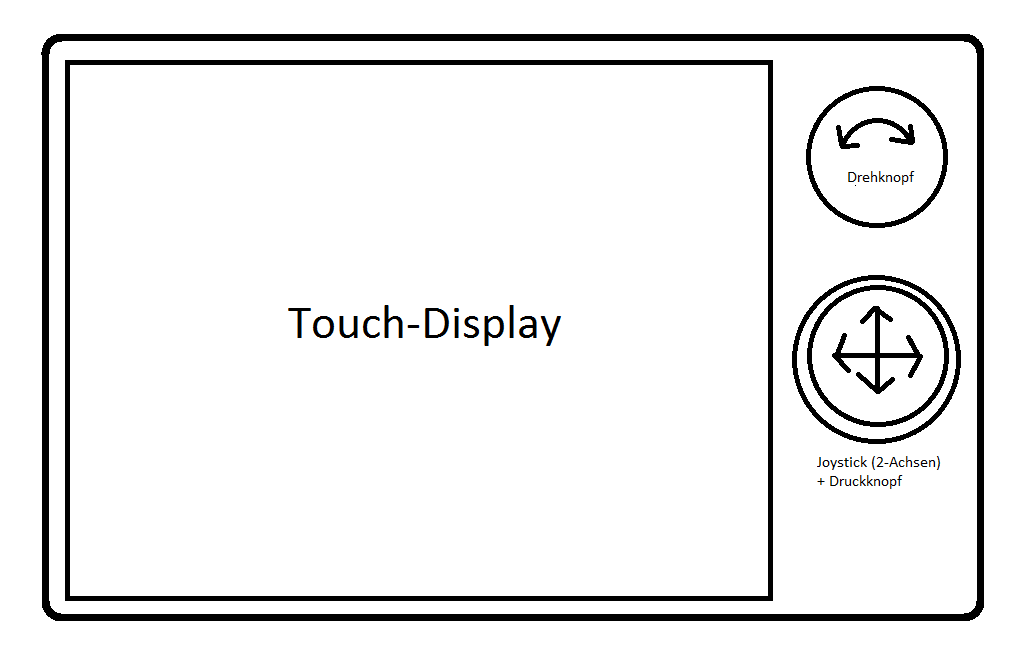
\includegraphics[scale=0.6]{Zettel1Aufg1-Steuer.png}
	\item Das Navigationsgerät ist mit lediglich drei Eingabeelementen mechanisch sehr einfach strukturiert. Den größten Teil des Gerätes nimmt der Touchscreen ein, flankiert wird er zur rechten Seite mit einem Drehknopf (auch als Druckknopf nutzbar) sowie einem 2-Achsen-Joystick (ebenfalls als Druckknopf nutzbar).
	
	Beim Betrachten der Umgebungsbedingungen, in welchen das Gerät hauptsächlich genutzt werden wird fallen unter anderem die feuchte bzw. nasse Umgebung (Kanu auf Meer) sowie die Außentemperatur um oder unter dem Nullpunkt auf. Das Gerät ist robust konstruiert und vollständig Wasserdicht, so dass auch ein regelmäßiges Kentern des Kanus keine Gefahr für die Elektronik darstellt. Da in nassen Umgebungen kapazitive Touchscreens sehr fehleranfällig sind, wird hier auf ein resistives Modell zurückgegriffen, welches im Notfall auch per Stift bedient werden kann. Da bei den Temperaturen, in welchen das Gerät zum Einsatz kommt i.d.R. Handschuhe getragen werden, sind die zwei Bedienelemente groß und griffig angelegt.
	
	Die Zieleingabe erfolgt entweder in Koordinatenform oder in Form von Ortsnamen über eine große Bildschirmtastatur. Die komplette Menüführung (und Tastaturbedienung) ist sowohl per Touch-Screen als auch mittels der beiden Bedienelemente möglich. Während der Fahrt wird stets ein Kartenausschnitt, welcher auf den Kanufahrer selbst zentriert ist, angezeigt. Hierfür kommt problemlos GPS zum Einsatz, da auf dem Meer wenig Beeinträchtigungen durch Bäume oder andere Hindernisse zu erwarten sind. Wahlweise werden außerdem im 9-Zoll-Display weitere Informationen wie Datum, Uhrzeit, Aktueller Kurs, Kurs zum Ziel, Weg zum Ziel, ggf. eingegebene Wegpunkte etc. angezeigt. 
	
	Auch an die Linkshänder unter den Inuit ist gedacht: Durch eine Einstellung lässt sich das Display um 180 Grad drehen, so dass die Bedienelemente auf der linken Seite angeordnet sind. 
\end{enumerate}

\end{document}
